\section{Diagramas de secuencia de la Iteración II}

\par A lo largo de esta sección se muestran los diagramas de secuencia de los casos de uso de la iteración II. Cabe decir, que para cada diagrama de secuencia se sobreentiende que el coche debe estar arrancado y los subsistemas a utilizar deben estar activados.

\par El diagrama de secuencia  en la figura \ref{img:vibrar_volante} hace referencia al \nameref{tab:CDUE-03}. Se muestra el \textit{flujo de ejecución normal} en el que el sistema es capaz de leer las líneas del carril y comparar si el vehículo está circulando con una trayectoria correcta. La segunda parte del cuadro \textit{alt} muestra el \textit{flujo de ejecución alternativo} en el que se produce la vibración del volante cuando no se siga la trayectoria correcta.

\begin{figure}[h]
  \begin{center}
    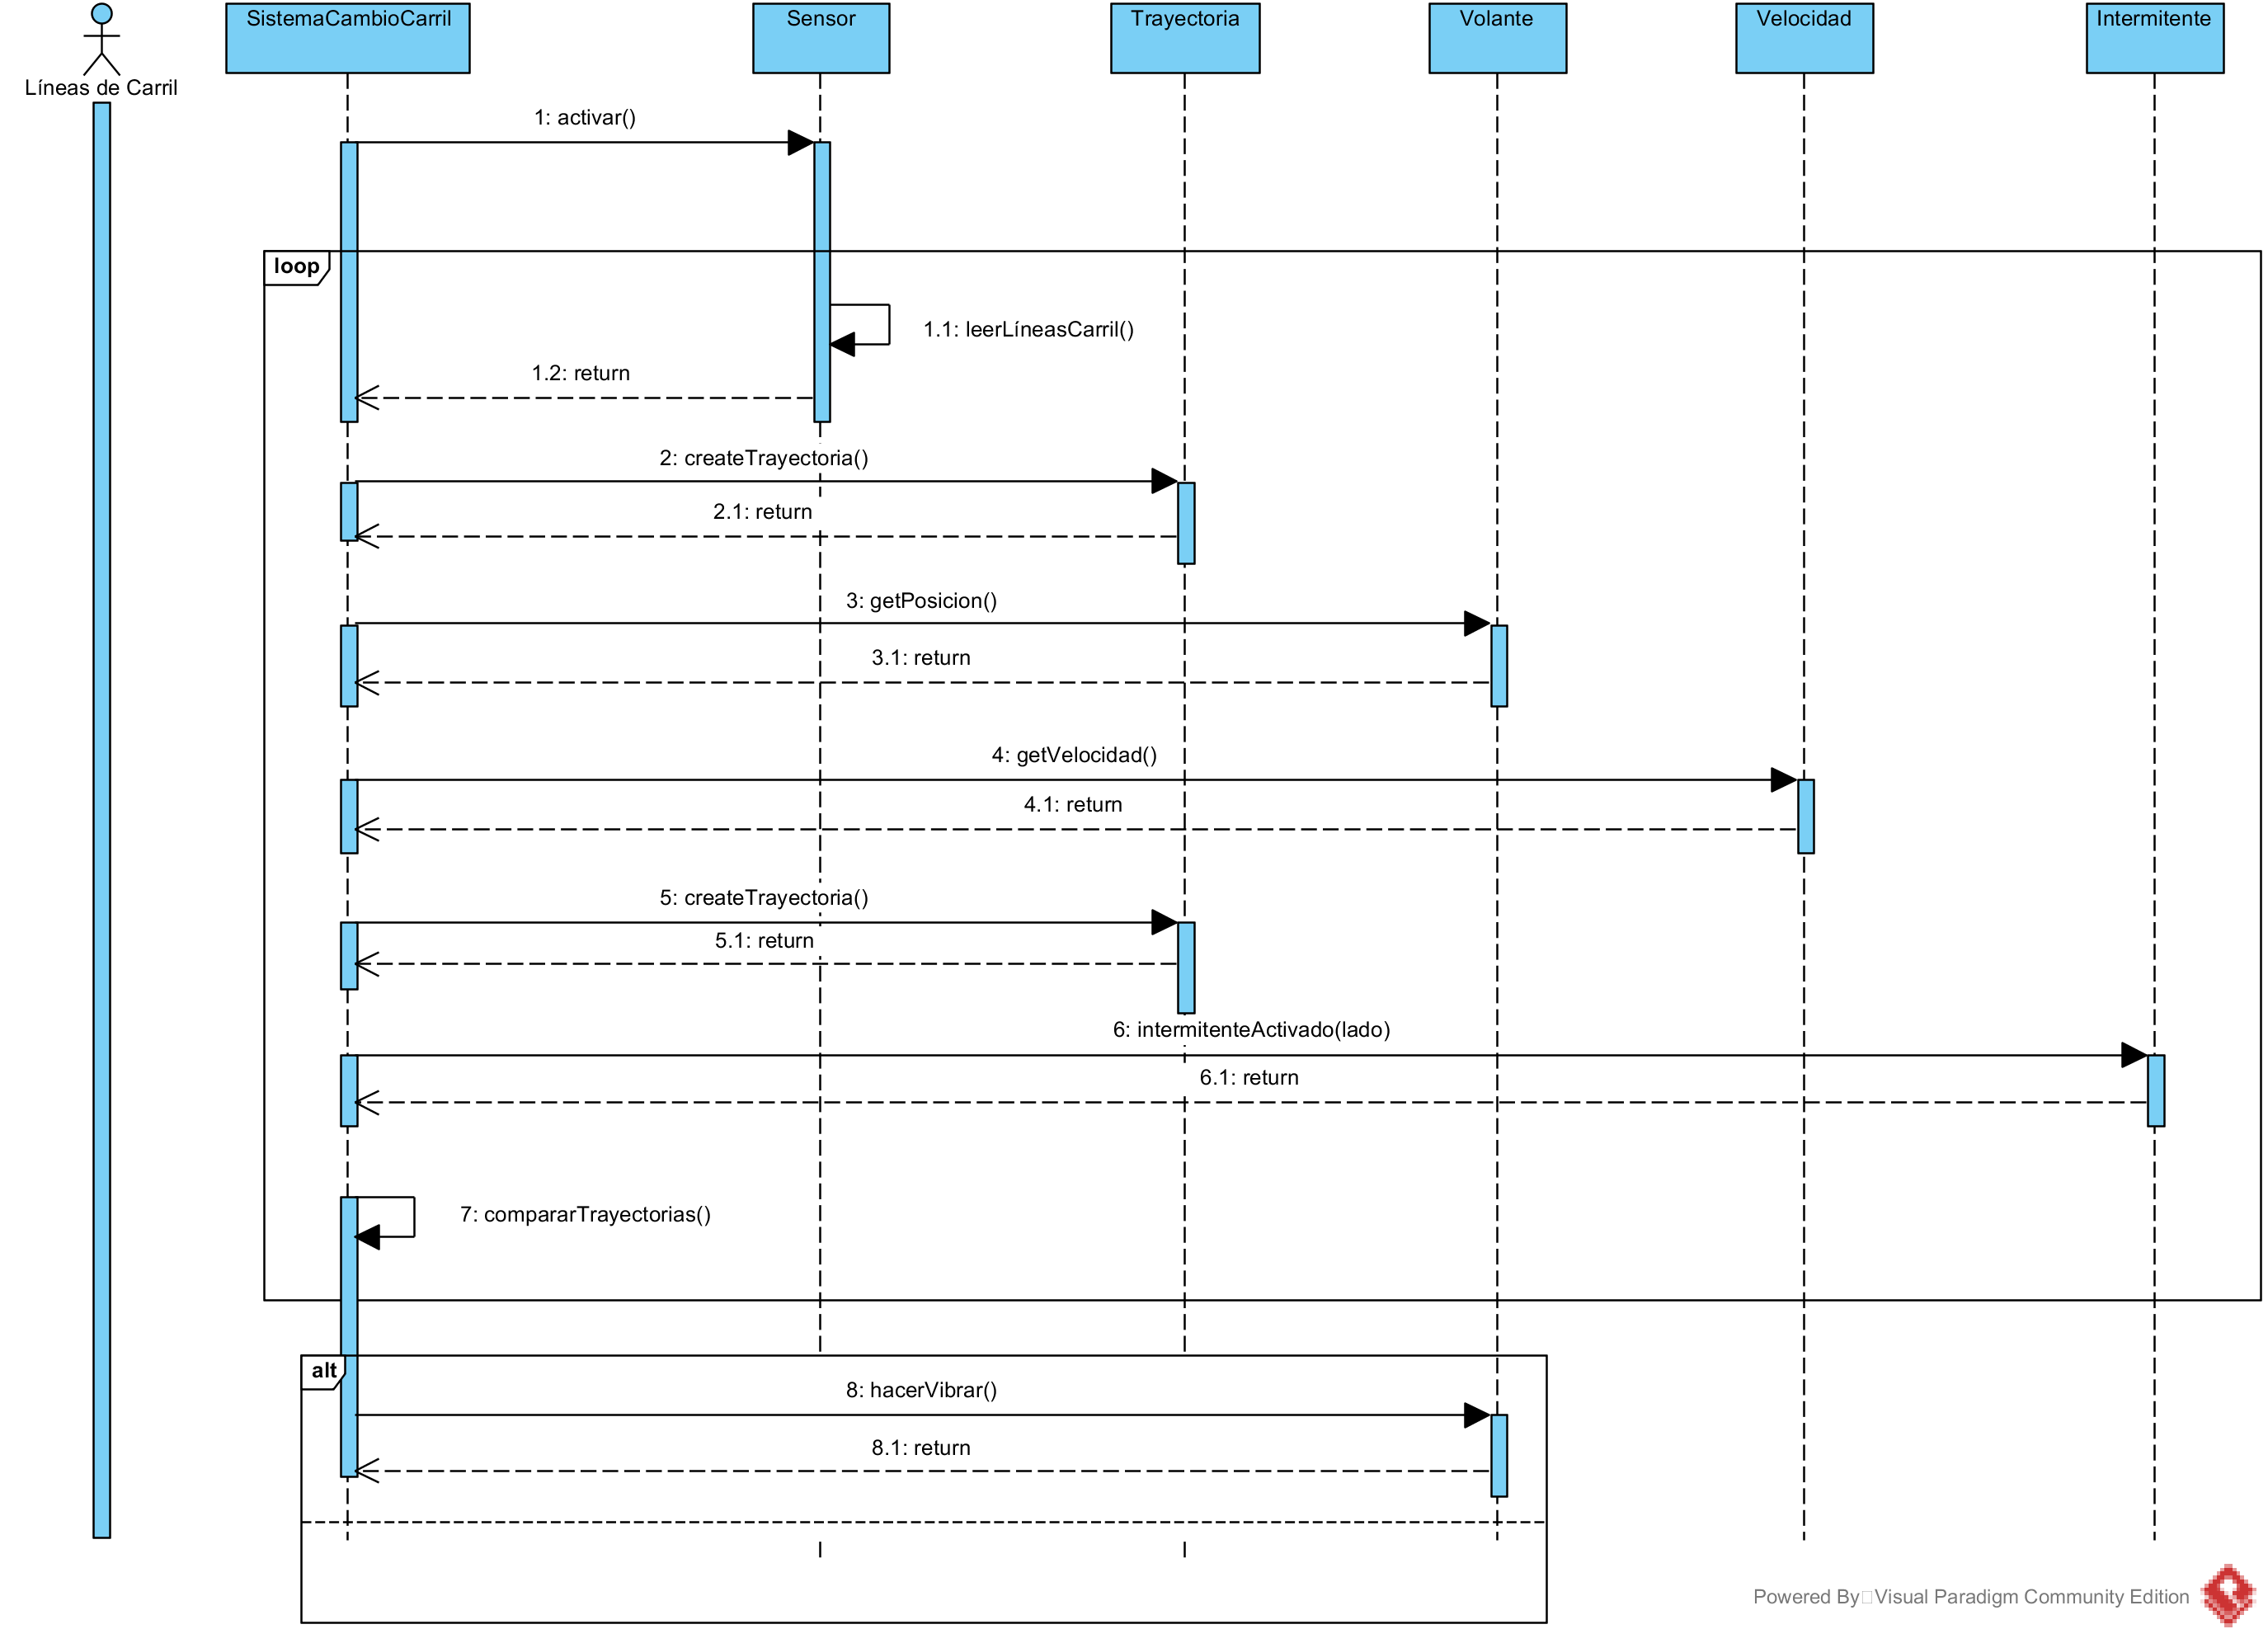
\includegraphics[width=0.75\textwidth]{./img/diagramas_de_secuencia/CDUE-03.png}
  \end{center}
  \caption{Diagrama de secuencia para el CDUE-03: \textit{Hacer vibrar el volante}}
  \label{img:vibrar_volante}
\end{figure}


\par El diagrama de secuencia  en la figura \ref{img:corregir_volante} hace referencia al \nameref{tab:CDUE-04}. Se muestra el \textit{flujo de ejecución normal} en el que el sistema es capaz de leer las líneas del carril y comparar si el vehículo está circulando con una trayectoria correcta. La primera parte del cuadro \textit{alt} muestra el \textit{flujo de ejecución alternativo} en el que se produce la corrección del volante cuando no se siga la trayectoria correcta.

\clearpage

\begin{figure}[h]
  \begin{center}
    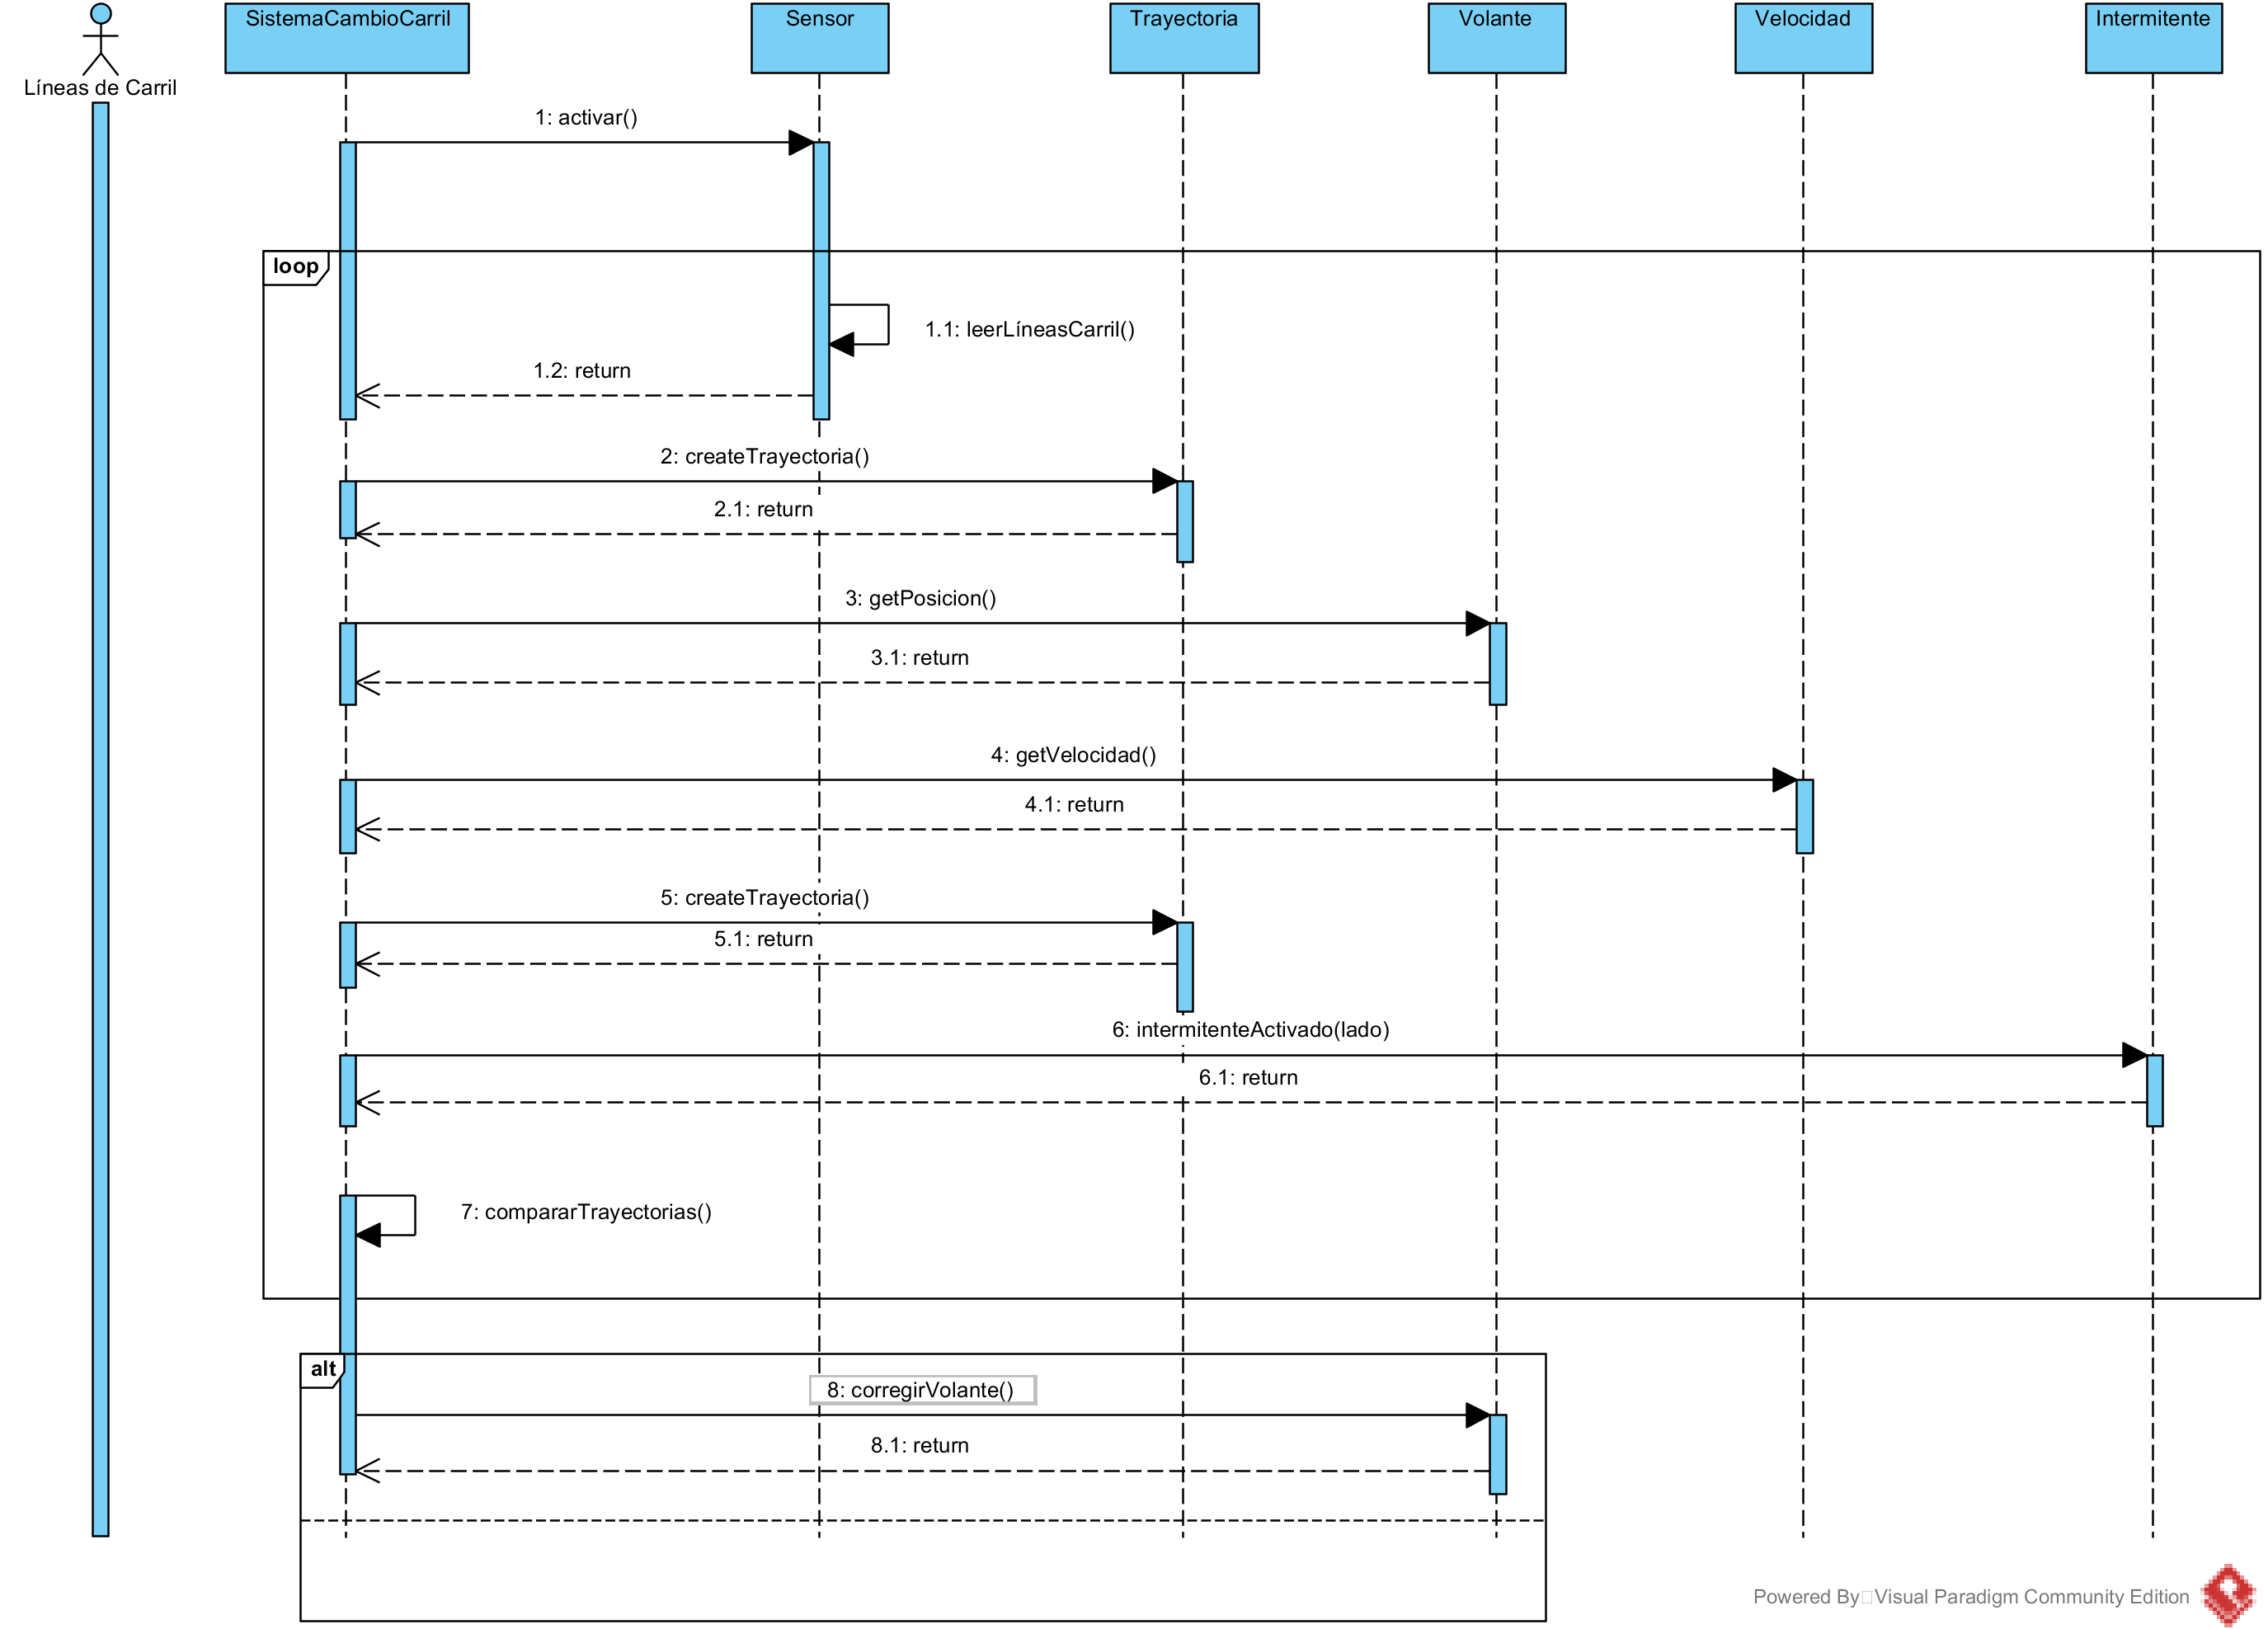
\includegraphics[width=0.75\textwidth]{./img/diagramas_de_secuencia/CDUE-04.png}
  \end{center}
  \caption{Diagrama de secuencia para el CDUE-04: \textit{Corregir el volante}}
  \label{img:corregir_volante}
\end{figure}

\par El diagrama de secuencia  en la figura \ref{img:limite_velocidad} hace referencia al \nameref{tab:CDUE-06}. Se muestra el \textit{flujo de ejecución normal} en el que el sistema es capaz de interpretar las señales en la primera parte del cuadro \textit{alt} de la figura. La segunda parte del cuadro \textit{alt} muestra el \textit{flujo de ejecución alternativo} en el que la velocidad máxima se comprueba gracias a la posición GPS. Segudamente, el sistema compara la velocidad máxima permitida y la velocidad a la que circula el vehículo, y se reduce la velocidad frenando el vehículo.

\begin{figure}[h]
  \begin{center}
    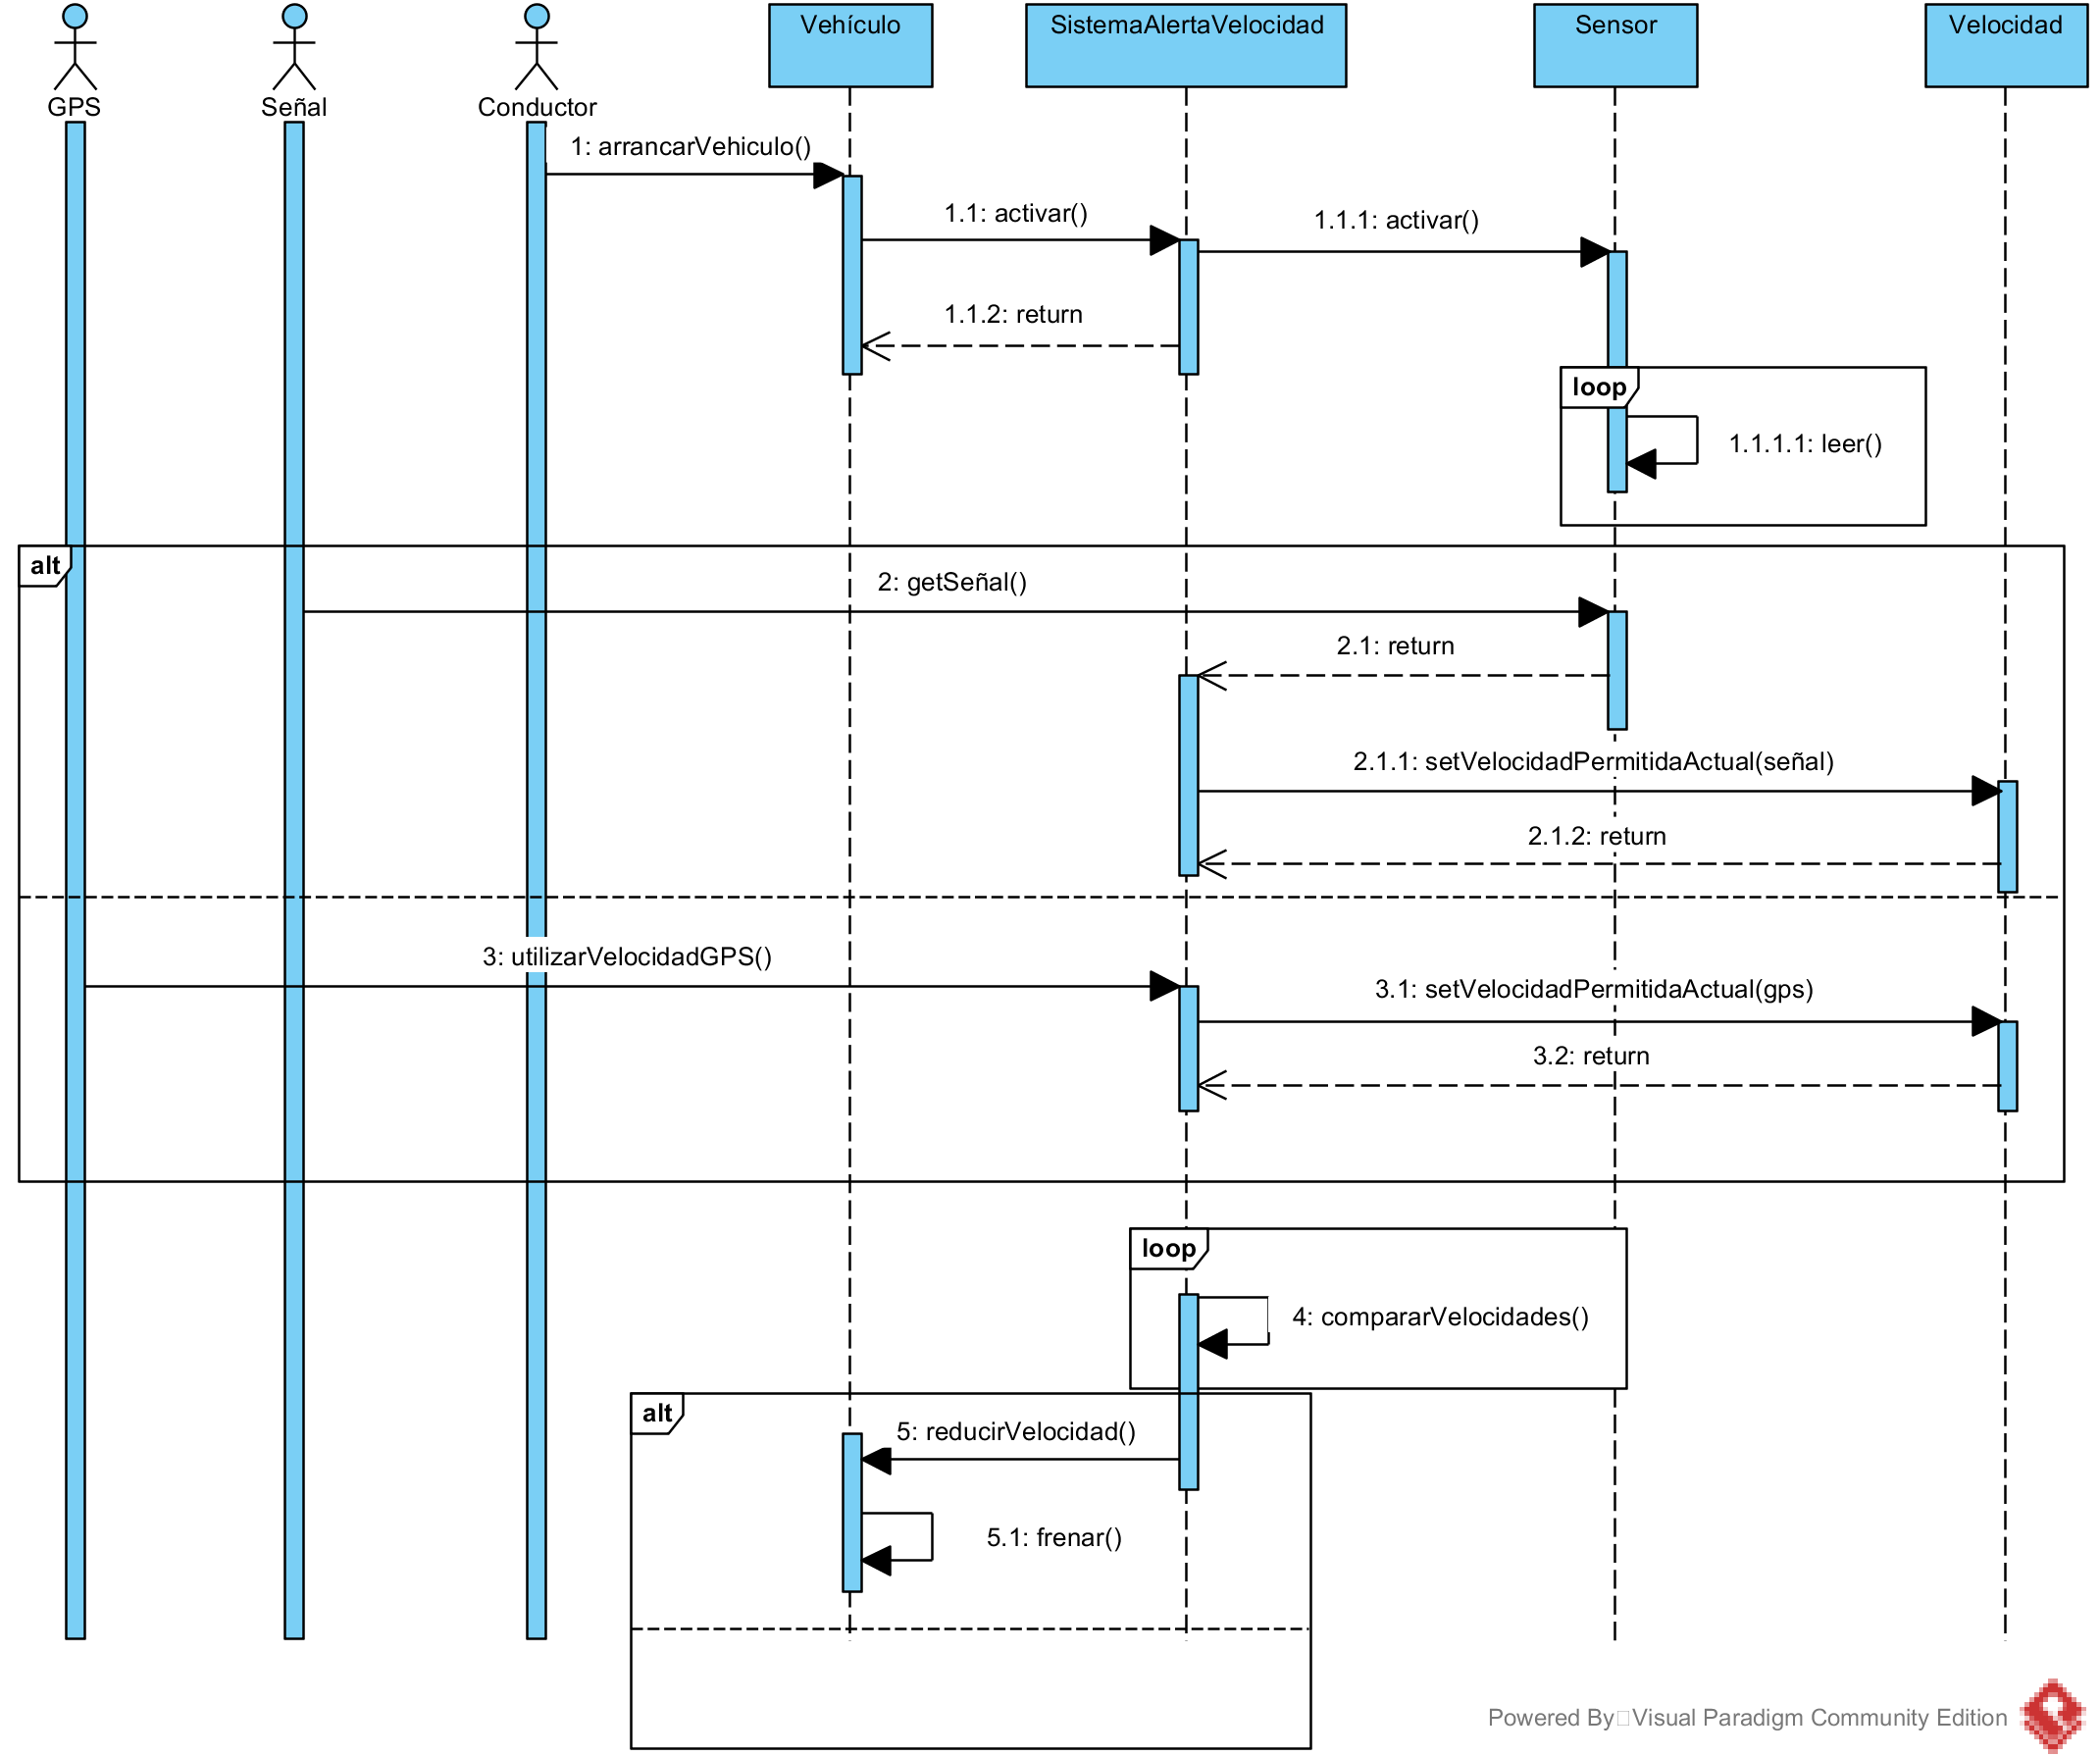
\includegraphics[width=0.75\textwidth]{./img/diagramas_de_secuencia/CDUE-06.png}
  \end{center}
  \caption{Diagrama de secuencia para el CDUE-06: \textit{No Superar Límite de Velocidad}}
  \label{img:limite_velocidad}
\end{figure}


\par El diagrama de secuencia  en la figura \ref{img:noti_descanso} hace referencia al \nameref{tab:CDUE-08}. Se muestra el \textit{flujo de ejecución normal} en el que el sistema es capaz de interpretar las expresiones faciales del conductor. Finalmente, se activara una notificación cuando el sistema detecte que el conductor está cansado, tal y como indica el recuadro \textit{alt}.

\begin{figure}[h]
  \begin{center}
    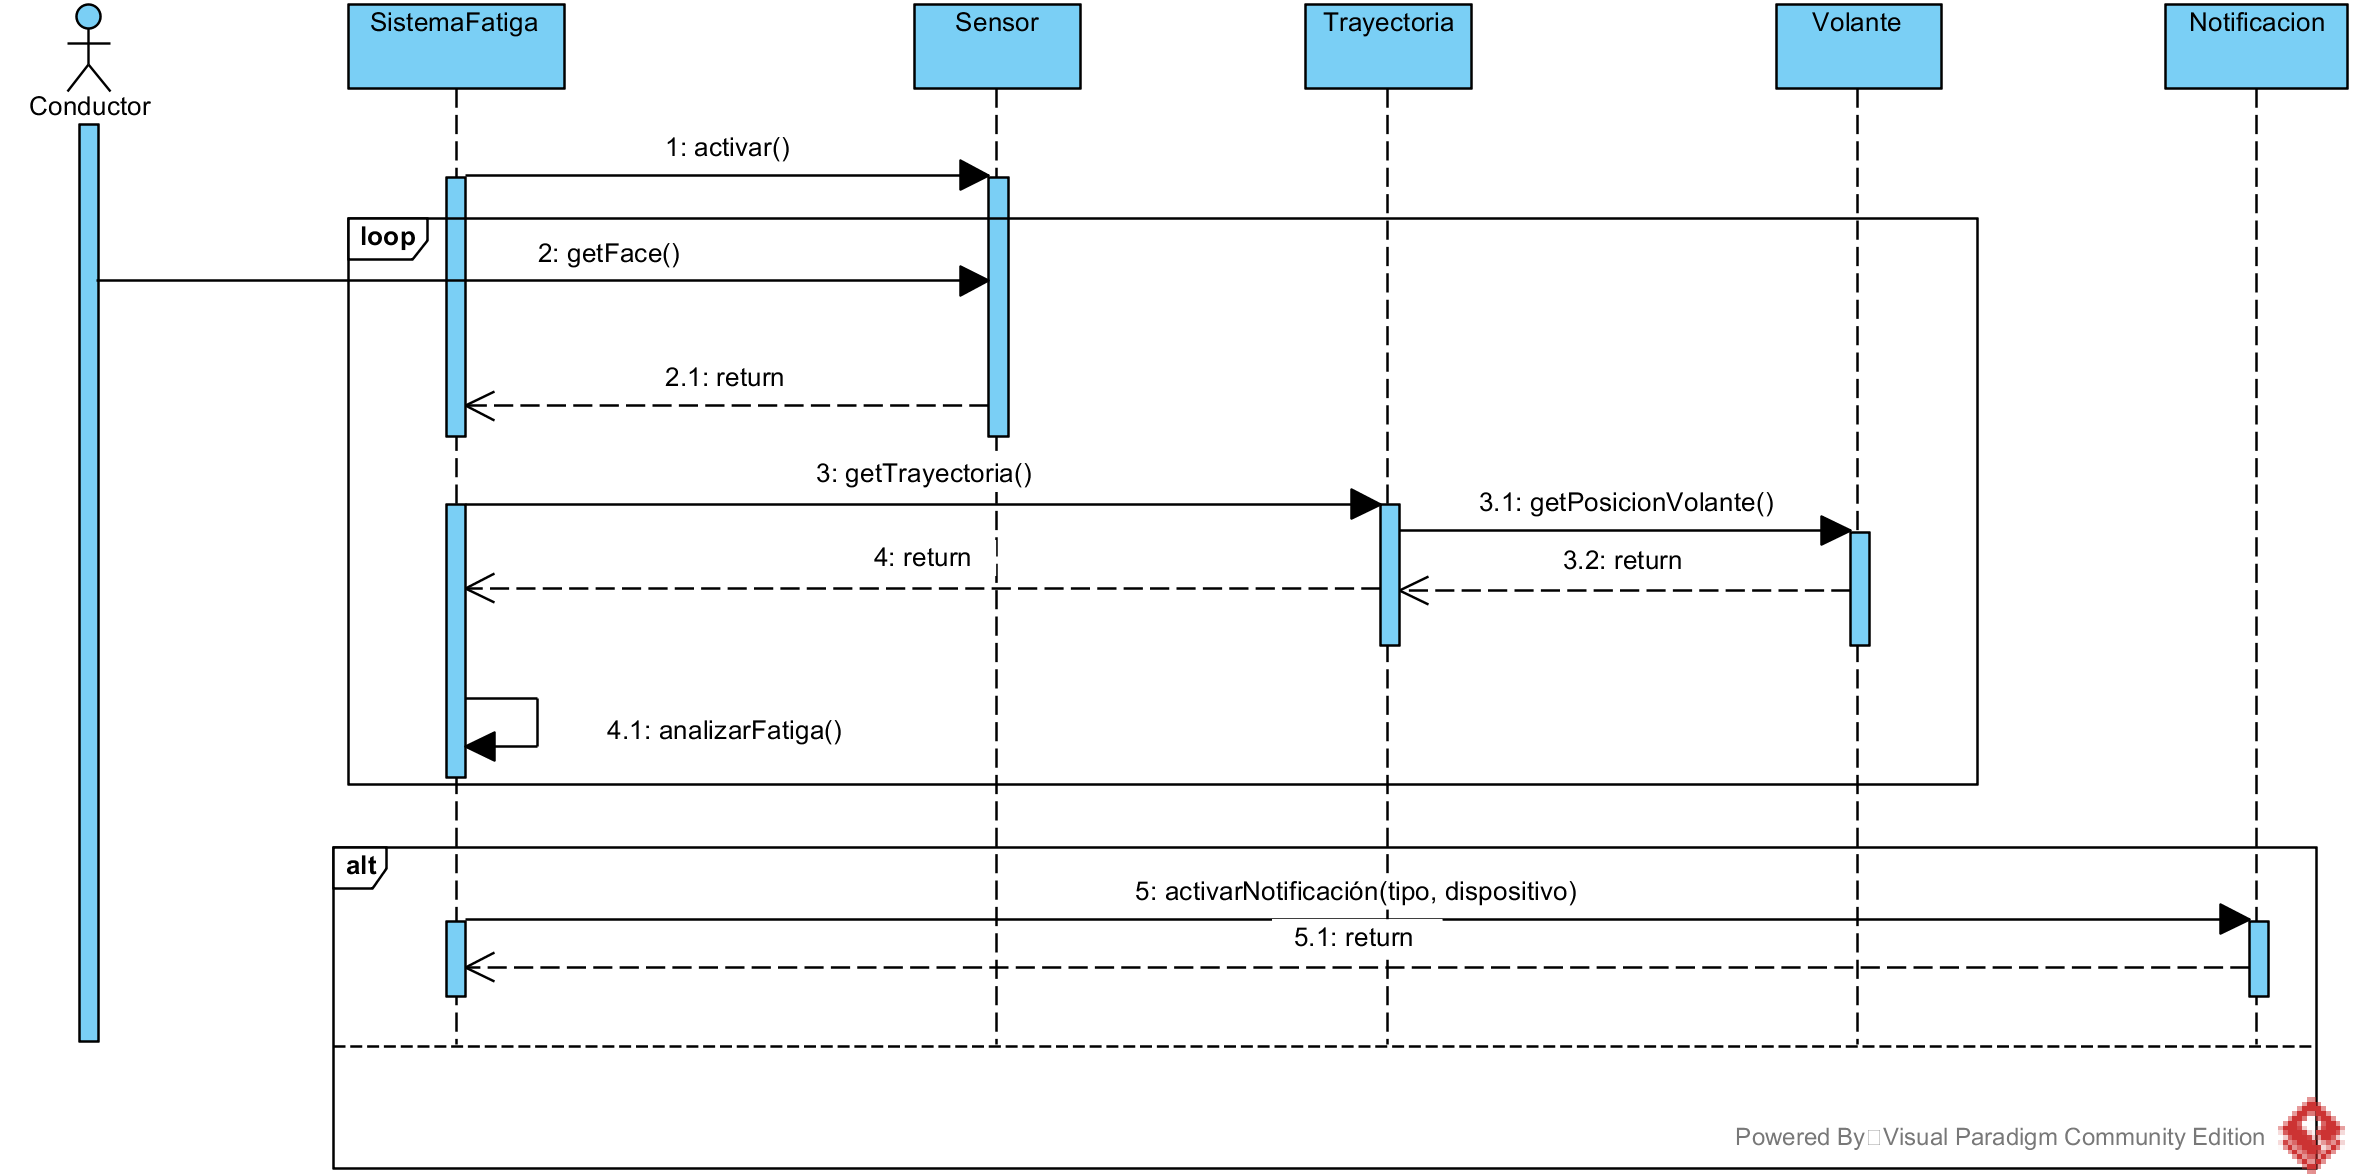
\includegraphics[width=0.75\textwidth]{./img/diagramas_de_secuencia/CDUE-08.png}
  \end{center}
  \caption{Diagrama de secuencia para el CDUE-08: \textit{Activar Notificación de Descanso}}
  \label{img:noti_descanso}
\end{figure}
